\documentclass{beamer}
\usepackage[english]{babel}
\usepackage[T1]{fontenc}
\usepackage[utf8]{inputenc} 
\usepackage{color} 
\usepackage{graphicx}
\graphicspath{{figures/}}

%\usepackage{subfig}

\usepackage{fixltx2e}
%\usepackage{url}

%\addto\captionsngerman{
%  \renewcommand{\figurename}{Abb.} %Abbildung -> Abb.
%  \renewcommand{\tablename}{Tab.} %Tabelle -> Tab.
%}

\usepackage{textcomp}

\definecolor{gray}{gray}{0.5}
\definecolor{key}{rgb}{0,0.5,0}
\usepackage{listings}
\lstset{%
    language=C, 
    breaklines=true,
    captionpos=b,
    tabsize=2,
    basicstyle=\ttfamily\small\setstretch{1},
    stringstyle=\color{red},
    showstringspaces=false,
    keywordstyle=\color{blue},
    emphstyle=\color{black}\bfseries,
    emphstyle=[2]\color{green},
    emphstyle=[3]\color{blue},
    upquote=true,
    commentstyle=\color{gray}\slshape,
    emphstyle=[4]\color{blue},
    breaklines=true,
    breakatwhitespace=true,
    numbers=left,
    numberstyle=\tiny,
    stepnumber=5,
    numberfirstline,
    numbersep=5pt,
    firstnumber=1
}

\usepackage[activate]{pdfcprot}
\pdfadjustspacing=1
\usepackage{thumbpdf}
%\usepackage[
%  pdftex,
%  pdfpagelabels,
%  plainpages=false,
%  colorlinks,
%  bookmarks         = true,
%  bookmarksopen     = true, % Bookmarks anzeigen...
%  pdftitle          = {ULE Scheduler},
%  pdfauthor         = {Stefan Sydow}
%]{hyperref}

%\beamersetuncovermixins{\opaqueness<1>{25}}{\opaqueness<2->{15}}
%\usetheme{Malmoe}
%\usetheme{Boadilla}
%\usecolortheme{beaver}
%\usecolortheme{seahorse}
\usecolortheme{dove}

\beamertemplatenavigationsymbolsempty
\setbeamertemplate{footline}[frame number]

\title{Model Slicing and Support Structure Generation for 3d Printing}  
\author[St. Sydow]{Stefan Sydow}
\institute[CG -- TU Berlin]{%
	Technische Universität Berlin\\
	Fakultät IV (Elektrotechnik und Informatik)\\
	Institut für Technische Informatik und Mikroelektronik\\
	Computer Graphics}
\titlegraphic{
\includegraphics[width=1.5cm]{tu-logo}}
\date{\today} 

\begin{document}
\begin{frame}
\titlepage
\end{frame} 

\begin{frame}
\frametitle{Agenda}
\tableofcontents
\end{frame} 

\section{Starting Point}
\begin{frame}
\frametitle{Starting Point} 
\begin{itemize}
 \item Many nice tools of libraries, but none suitable.\\
     (pythonOCC, Meshlab, libcarve, netfabb, FreeCAD)
 \item Slicing software like Skeinfrogde and Slic3r are very complex.
 \item Own C++ raytracer implementation.
\end{itemize}
\end{frame}

\section{Architecture}
\begin{frame}
\frametitle{Architecture} 
 \begin{itemize}
  \item import model; build KD-tree.
  \item Generate support structure.
  \item slice model; build contours.
  \item fill contours with an adaptive grid.
 \end{itemize}
\begin{figure}
\centering
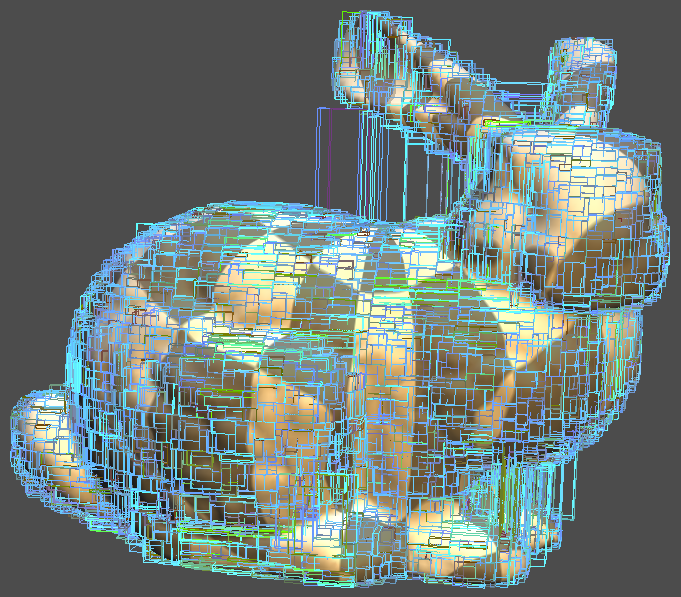
\includegraphics[width=0.5\textwidth]{kdtree}
\caption{Last level of the KD-tree.}
\end{figure}
\end{frame}

\section{Implementation}

\subsection{Support Structur Generation}
\begin{frame}
\frametitle{Support Structur Generation} 
 \begin{itemize}
  \item Mark triangles faceing steep ``down''.
  \item Obtain the contour of this surface.
  \item Projekt onto the model and the base plane.
  \item Build the support volume from support and projection surface.
  \item Use the KD tree representation for slicing.
 \end{itemize}
\begin{figure}
\centering
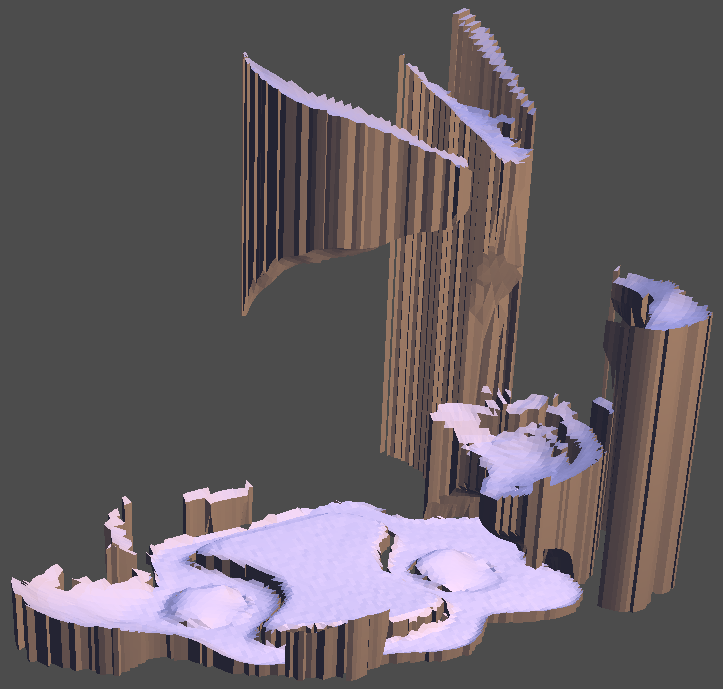
\includegraphics[width=0.45\textwidth]{support_mesh}
\caption{Support volume for the Stanford Bunny.}
\end{figure}
\end{frame}

\subsection{Slicing}
\begin{frame}
\frametitle{Slicing} 
 \begin{itemize}
  \item Intersect model and support KD tree with the slicing plane
  \item Build contour set form edges.
 \end{itemize}
\begin{figure}
\centering
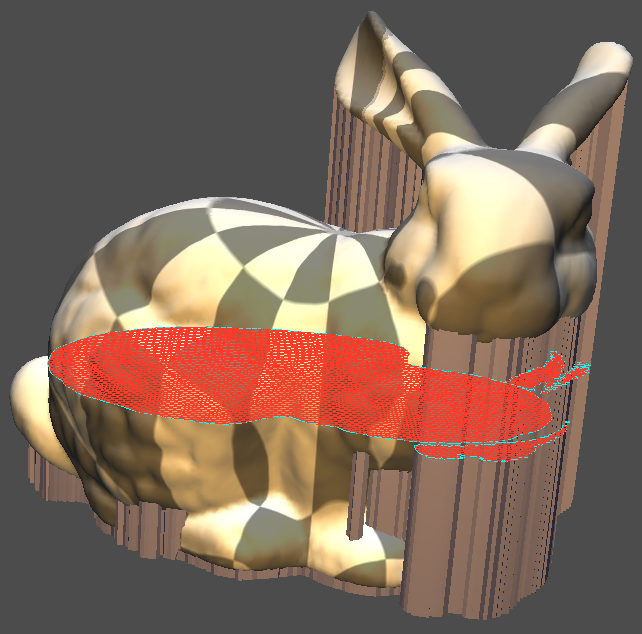
\includegraphics[width=0.6\textwidth]{slice}
\caption{Slice through the model}
\end{figure}
\end{frame}

\subsection{Adaptive Mesh}
\begin{frame}
\frametitle{Adaptive Mesh} 
 \begin{itemize}
  \item Grid layout is defined by a set of planes.
  \item Planes are translated along their normal to generate different lines.
  \item Translation step decides on grid density
  \item $ds = ds_{max} \cdot \left(1 - \frac{h_{max}}{h_{line avg}}\right)$ \\
      $h$ : model height; $ds$ : translation step
 \end{itemize}
\begin{figure}
\centering
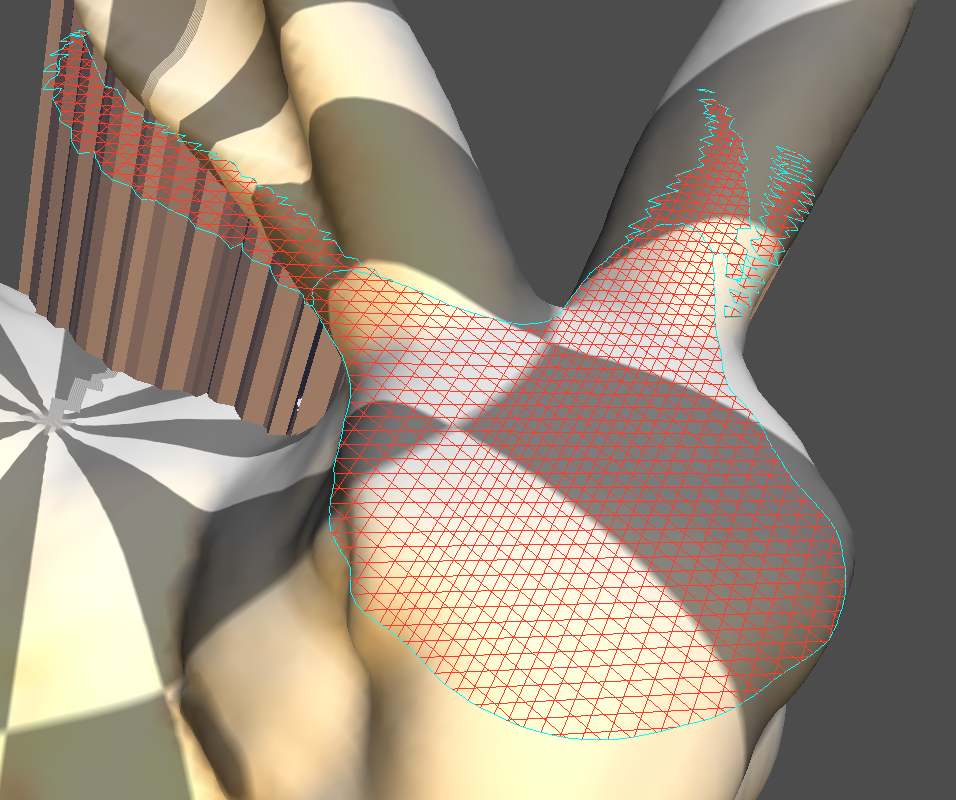
\includegraphics[width=0.45\textwidth]{slice1}
\caption{Adaptive grid density}
\end{figure}
\end{frame}
\end{document}
